\subsection{(a) & (b) & (c)}

I estimate the equation in problem 1 (a) by including only second lags (specification 1) and by including second and third lags (specification 2). Specification 3 is autocorrelated transmitted shocks without fixed effects (the selected $\rho=0.758$) and specification 4 (the selected $\rho=1.159$) is autocorrelated transmitted shocks with fixed effects.


\begin{figure}[h!]
    \centering
    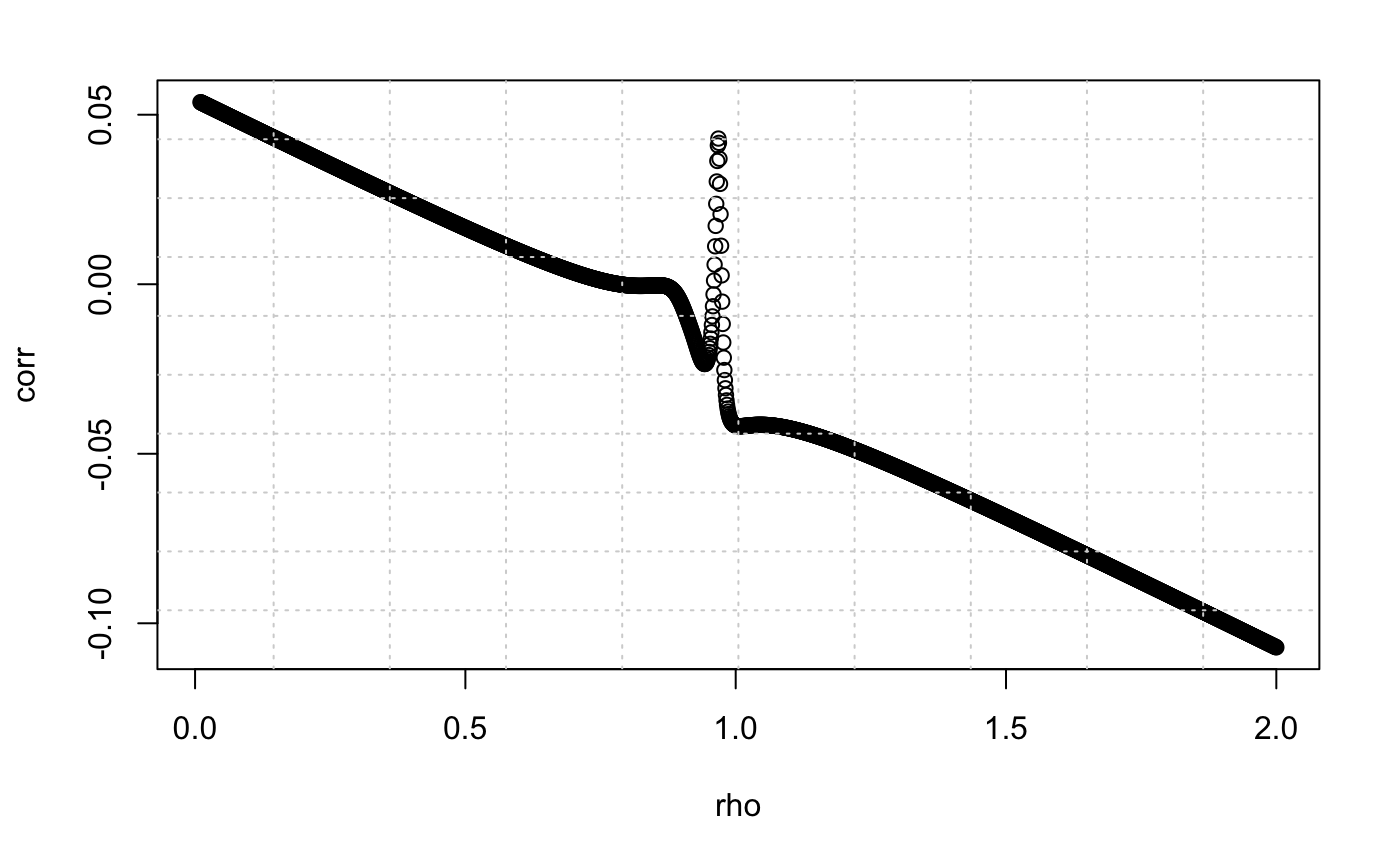
\includegraphics[scale=0.15]{HW2/Attachments/Q1b.png}
    \caption{Moment Condition vs $\rho$ for (b)}
    \label{fig:my_label}
\end{figure}

\begin{figure}[h!]
    \centering
    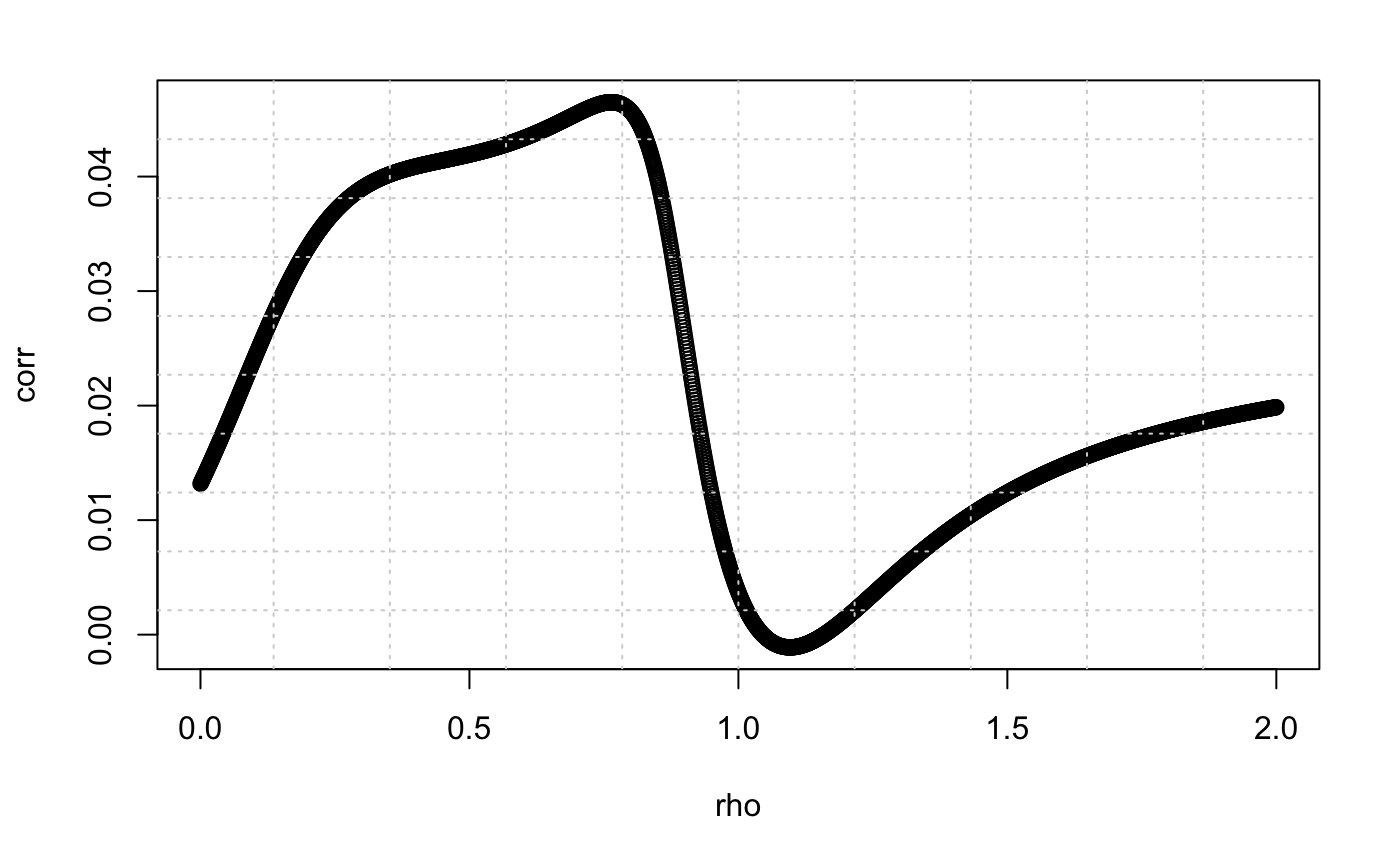
\includegraphics[scale=0.15]{HW2/Attachments/Q1c.png}
    \caption{Moment Condition vs $\rho$ for (c)}
    \label{fig:my_label}
\end{figure}

\begin{table}[h!]
    \centering
    \footnotesize{
    {
\def\sym#1{\ifmmode^{#1}\else\(^{#1}\)\fi}
\begin{tabular}{l*{4}{c}}
\hline\hline
            &\multicolumn{1}{c}{(1)}&\multicolumn{1}{c}{(2)}&\multicolumn{1}{c}{(3)}&\multicolumn{1}{c}{(4)}\\
            &\multicolumn{1}{c}{IV Regressions with 2L}&\multicolumn{1}{c}{IV Regressions with 3L}&\multicolumn{1}{c}{AR Shocks}&\multicolumn{1}{c}{AR Shocks+FE}\\
\hline
lemp        &       0.221         &       0.661         &       0.517\sym{***}&      -1.076         \\
            &      (0.68)         &      (1.85)         &      (3.65)         &     (-0.25)         \\
[1em]
ldnpt       &       0.869\sym{**} &      -0.269         &       0.439\sym{***}&       4.013         \\
            &      (2.78)         &     (-0.68)         &      (4.54)         &      (0.56)         \\
[1em]
ldrst       &      -0.555         &       0.409         &      0.0963         &       0.221         \\
            &     (-1.70)         &      (1.34)         &      (1.32)         &      (0.03)         \\
[1em]
d73         &           0         &           0         &           0         &           0         \\
            &         (.)         &         (.)         &         (.)         &         (.)         \\
[1em]
d78         &           0         &           0         &           0         &           0         \\
            &         (.)         &         (.)         &         (.)         &         (.)         \\
[1em]
d83         &      -0.633\sym{***}&           0         &      -0.390\sym{***}&           0         \\
            &     (-4.46)         &         (.)         &    (-11.21)         &         (.)         \\
[1em]
d88         &           0         &           0         &           0         &           0         \\
            &         (.)         &         (.)         &         (.)         &         (.)         \\
[1em]
d357\_73     &           0         &           0         &           0         &           0         \\
            &         (.)         &         (.)         &         (.)         &         (.)         \\
[1em]
d357\_78     &           0         &           0         &           0         &           0         \\
            &         (.)         &         (.)         &         (.)         &         (.)         \\
[1em]
d357\_83     &       1.471\sym{***}&           0         &       0.853\sym{***}&           0         \\
            &     (13.80)         &         (.)         &     (16.92)         &         (.)         \\
[1em]
d357\_88     &       1.087\sym{***}&       0.903\sym{***}&       0.810\sym{***}&      -0.798         \\
            &     (10.69)         &      (8.71)         &     (15.09)         &     (-0.75)         \\
[1em]
\_cons      &       0.474\sym{***}&       0.161         &       0.820\sym{***}&       1.959         \\
            &      (4.66)         &      (1.66)         &     (10.55)         &      (0.68)         \\
\hline
\(N\)       &         682         &         214         &         682         &         214         \\
\hline\hline
\multicolumn{5}{l}{\footnotesize \textit{t} statistics in parentheses}\\
\multicolumn{5}{l}{\footnotesize \sym{*} \(p<0.05\), \sym{**} \(p<0.01\), \sym{***} \(p<0.001\)}\\
\end{tabular}
}

    }
    \caption{Question 1}
    \label{tab:my_label}
\end{table}

\subsection{(d)}

In Table (1), we can the see results for different settings. In  specifications (1) and (2) the coefficient on R\&D capital and the coefficient on capital is negative, which does not make much of sense. Checking the first stage regression F-statistic, we see that the 2-lagged and 3-lagged inputs are not very good IVs.

Moreover, the results of specification (3) seem much more reasonable suggesting that the assumption of no autocorrelation in the transmitted shock is important. The estimated autocorrelation is $\rho=0.758$, which is a high coefficient, so ignoring it results in a seriously biased estimates.

Also, specification (4) suggest that nothing is significant. We should notice that including fixed effects makes us use only balanced panel for estimation, reducing the sample size threefold. Moreover, we have to use higher-order lags for estimation which makes them weaker instruments. Therefore, in this case, having firm fixed effects creates more problems and makes the inference harder.
